\documentclass[11pt]{article}
\usepackage[margin=1in]{geometry}
\usepackage{mathpazo}
\usepackage{amsmath,amssymb}
\usepackage{microtype}
\usepackage{booktabs}
\usepackage{graphicx}
\usepackage[dvipsnames]{xcolor}
\usepackage{tikz}
\usetikzlibrary{positioning,arrows.meta,calc,fit,backgrounds}
\usepackage[most]{tcolorbox}
\usepackage{enumitem}
\usepackage{listings}
\usepackage[font=small,labelfont=bf]{caption}
\usepackage{hyperref}
\hypersetup{colorlinks=true,linkcolor=MidnightBlue,citecolor=MidnightBlue,urlcolor=MidnightBlue}
\usepackage{cleveref}
\urlstyle{tt}
\def\UrlBreaks{\do\_\do/\do.}
\newcommand{\file}[1]{\nolinkurl{#1}}
\newcommand{\code}[1]{\texttt{#1}}
\newcommand{\mhh}{m_{hh}}
\newcommand{\bw}{\boldsymbol{\omega}}
\newcommand{\bp}{\boldsymbol{p}}
\newcommand{\bx}{\boldsymbol{x}}
\newcommand{\data}{\mathcal{D}}

\definecolor{trainable}{HTML}{1B6CA8}
\definecolor{physics}{HTML}{2E933C}
\definecolor{datac}{HTML}{7B4EA3}
\definecolor{warn}{HTML}{C0392B}

\newtcolorbox{keyidea}[1][]{enhanced,breakable,colback=physics!6,colframe=physics!70!black,
  fonttitle=\bfseries,title={#1},boxrule=0.6pt,arc=2pt,left=6pt,right=6pt}
\newtcolorbox{aside}[1][]{enhanced,breakable,colback=trainable!5,colframe=trainable!70!black,
  fonttitle=\bfseries,title={#1},boxrule=0.6pt,arc=2pt,left=6pt,right=6pt}
\newtcolorbox{assume}[1][]{enhanced,breakable,colback=datac!5,colframe=datac!70!black,
  fonttitle=\bfseries,title={#1},boxrule=0.6pt,arc=2pt,left=6pt,right=6pt}
\newtcolorbox{watch}[1][]{enhanced,breakable,colback=warn!5,colframe=warn!70!black,
  fonttitle=\bfseries,title={#1},boxrule=0.6pt,arc=2pt,left=6pt,right=6pt}
\setlist{itemsep=2pt,topsep=3pt}
\setlength{\emergencystretch}{3em}

\lstset{language=Python, basicstyle=\ttfamily\small, columns=fullflexible,
  keepspaces=true, commentstyle=\color{physics!70!black}\itshape,
  keywordstyle=\color{trainable!90!black}\bfseries, stringstyle=\color{datac},
  showstringspaces=false, frame=single, rulecolor=\color{gray!40},
  backgroundcolor=\color{gray!3}, xleftmargin=4pt, xrightmargin=4pt,
  aboveskip=6pt, belowskip=6pt}

\newcommand{\bbeta}{\boldsymbol{\beta}}
\newcommand{\bC}{\boldsymbol{C}}

\title{\textbf{The smooth $23\times80$ model}\\[4pt]
\large A continuous, exactly Bayesian model of $d\sigma/dm_{hh}$ as the primary surrogate\\[4pt]
\normalsize Plan, for review before any code is written}
\author{P.~Bhat, N.~De~Filippis, K.\,F.~Johnson, H.\,B.~Prosper, R.~Starnes}
\date{October 31, 2026}

\begin{document}
\maketitle

\begin{abstract}
\noindent
The free $23\times80$ fit, 23 numbers per $m_{hh}$ bin fitted by weighted least squares, is
as accurate as the network ensemble, its posterior is exactly Gaussian, and it needs no
training. Its weaknesses are that it exists only at the 80 bin centres, describes bin
integrals rather than the density $d\sigma/dm_{hh}$, and does not use the fact that the
coefficient functions are smooth. We propose to make it the primary model in a smooth form:
each coefficient function is written as a sum of spline basis functions, the likelihood
compares the \emph{integral} of the model over each bin with POWHEG, a smoothness prior with
strengths set by the evidence regularises the fit, and an optional threshold factor builds in
the phase-space behaviour at $m_{hh} = 2m_h$. The model stays linear in its parameters, so
the posterior, the predictions for any binning, the density at any $m_{hh}$ and their
uncertainties are all exact and cheap. Validation includes a new test of within-bin
accuracy: fit on 30-GeV bins, predict the 15-GeV bins. The decisions to be made are collected
in \cref{sec:decisions}.
\end{abstract}

\begin{keyidea}[The proposal in one paragraph]
$\displaystyle \frac{d\sigma}{dm}(m;\theta) = \sum_{i=1}^{23} C_i(\theta)\, a_i(m), \qquad
a_i(m) = \phi(m)\sum_{j=1}^{J}\beta_{ij}\, B_j(m)$, with $B_j$ cubic B-splines, $\phi$ an
optional threshold factor, and $23J$ parameters $\beta_{ij}$. The cross section in bin
$[e_k, e_{k+1}]$ is $\sum_{i,j} C_i(\theta)\,\beta_{ij}\,I_{jk}$ with
$I_{jk} = \int_{e_k}^{e_{k+1}}\phi B_j\,dm$, linear in $\bbeta$. Gaussian likelihood with the
exact Poisson variances; Gaussian smoothness prior on the second differences of each
$\beta_{i\cdot}$, its 23 strengths chosen by maximising the evidence; exact Gaussian
posterior; the cancellation-aware discrepancy added to the predictions.
\end{keyidea}

\tableofcontents

% ===========================================================================
\section{Why this model}
\label{sec:why}

\begin{itemize}
  \item \textbf{The network is not the limit.} The free $23\times80$ fit matches the ensemble
    on the test spectra (median $\chi^2/N$ 1.088 vs 1.085) and, with the cancellation-aware
    discrepancy, is equally well calibrated (pull s.d.\ 0.999 vs 1.004)
    (\file{docs/modelerror/new_error_model.pdf}). The remaining error is a mismatch between
    POWHEG and the 23-term form, which no model of that form can remove.
  \item \textbf{Linear is better, other things equal.} A model linear in its parameters has an
    exact Gaussian posterior: no Markov chains, no Laplace approximation, no random seeds, no
    ensemble. The uncertainty is a matrix inverse.
  \item \textbf{But the free fit has three defects.} (i) It is defined only at the bin
    centres; (ii) it models bin integrals, so reading it as $15\,\text{GeV}\times
    d\sigma/dm$ at the centre is an approximation (0.17\% of the value, 6\% of the noise, in
    the first ten bins); (iii) it treats the 80 values of each $a_i$ as unrelated, so its
    $a_i$ jitter from bin to bin and its poorly determined combinations
    ($a_{16}$--$a_{20}$) are not helped by their neighbours.
  \item \textbf{The network's interpolation is not to be trusted} between bin centres below
    600~GeV: the 20 networks disagree there twice as much as at the centres, because nothing
    in the data constrains them.
\end{itemize}

The smooth model removes the three defects and keeps linearity. The free fit is its limit
with one box-shaped basis function per bin and no prior (\cref{sec:limit}).

% ===========================================================================
\section{The model}
\label{sec:model}

\subsection{The density and the bins}

POWHEG gives, for each spectrum $s$ at HEFT point $\theta_s$, the cross section in bins of
15~GeV, $t_{sk} = \int_{e_k}^{e_{k+1}} \frac{d\sigma}{dm}(m;\theta_s)\,dm$ plus noise. We
model the density
\begin{equation}
  \frac{d\sigma}{dm}(m;\theta) = \sum_{i=1}^{23} C_i(\theta)\, a_i(m) ,
  \label{eq:density}
\end{equation}
with the same 23 monomials $C_i$ as \texttt{HEFTNet} (\file{docs/dihiggs_model.pdf}); here
$a_i(m)$ is a density, in pb/GeV. The model's prediction for bin $k$ is the integral of
\cref{eq:density} over the bin, never its value at the centre.

\subsection{The coefficient functions}

Each coefficient function is expanded in $J$ cubic B-splines on a fixed set of knots, times a
threshold factor:
\begin{equation}
  a_i(m) = \phi(m) \sum_{j=1}^{J} \beta_{ij}\, B_j(m) .
  \label{eq:spline}
\end{equation}

\begin{aside}[B-splines in brief]
A cubic B-spline $B_j(m)$ is a smooth bump, a piecewise cubic polynomial that is non-zero only
over four consecutive knot intervals and joins with continuous first and second derivatives.
A weighted sum of them can represent any smooth curve whose wiggles are not finer than the
knot spacing. Each coefficient $\beta_{ij}$ acts locally: it moves $a_i$ only near knot $j$.
They are the standard tool for smoothing in statistics (de Boor; Eilers \& Marx).
\end{aside}

\paragraph{Knots.} The functions change fastest just above threshold and slowly above
600~GeV (\file{docs/paper/fig_coefficients.pdf}). The knots should therefore be denser near
threshold. A simple choice is to space them uniformly in $u = \sqrt{m - 250\,\text{GeV}}$,
which places a third of them below about 400~GeV. With a smoothness prior
(\cref{sec:prior}) the exact number matters little as long as it is generous: we propose
$J = 40$ (920 parameters), and will check $J = 30$ and 60.

\paragraph{Threshold factor.} Near $m_{hh} = 2m_h = 250$~GeV the phase space of two Higgs
bosons vanishes like $\beta_h = \sqrt{1 - 4m_h^2/m^2}$, and so does $d\sigma/dm$ (for an
$s$-wave). Choosing $\phi(m) = \beta_h(m)$ builds this in, so the splines need only describe
the smooth remainder. The first 15-GeV bin (255--270~GeV) starts 5~GeV above threshold, so the
factor matters mostly there; we will compare $\phi = \beta_h$ with $\phi = 1$
(\cref{sec:decisions}).

\subsection{Linear in the parameters}

Collect the $23J$ coefficients into one vector $\bbeta$. The prediction for spectrum $s$ in
bin $k$ is
\begin{equation}
  f_{sk} = \sum_{i=1}^{23}\sum_{j=1}^{J} C_i(\theta_s)\, I_{jk}\, \beta_{ij}
         = \big(\bC(\theta_s) \otimes \boldsymbol I_k\big)^{\mathsf T}\bbeta,
  \qquad I_{jk} = \int_{e_k}^{e_{k+1}} \phi(m) B_j(m)\, dm ,
  \label{eq:linear}
\end{equation}
where $\boldsymbol I_k = (I_{1k},\dots,I_{Jk})$ and $\otimes$ is the Kronecker product. The
$80\times J$ numbers $I_{jk}$ depend only on the knots and the binning and are computed once,
accurately, by Gauss--Legendre quadrature (8 points per bin per spline piece).

\begin{figure}[h]
\centering
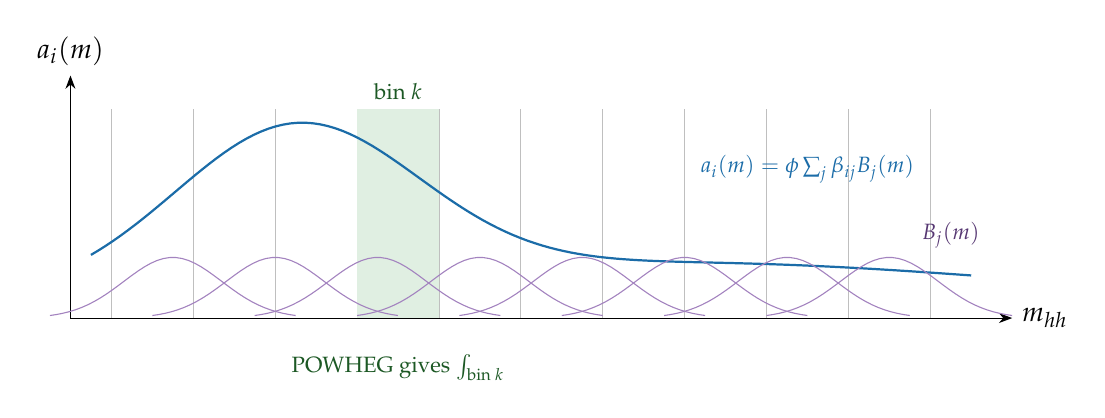
\begin{tikzpicture}[xscale=1.3, yscale=1.4, >=Stealth]
  \draw[->] (0,0) -- (9.2,0) node[right] {$m_{hh}$};
  \draw[->] (0,0) -- (0,2.2) node[above] {$a_i(m)$};
  \foreach \x in {0.4,1.2,2.0,2.8,3.6,4.4,5.2,6.0,6.8,7.6,8.4} \draw[gray!50] (\x,0) -- (\x,1.9);
  \fill[physics!15] (2.8,0) rectangle (3.6,1.9);
  \node[physics!60!black, font=\footnotesize] at (3.2,2.05) {bin $k$};
  \draw[trainable, thick, domain=0.2:8.8, samples=120] plot (\x, {0.15 + 1.45*exp(-0.35*(\x-2.2)^2) + 0.35*exp(-0.05*(\x-6)^2)});
  \foreach \c in {1.0,2.0,3.0,4.0,5.0,6.0,7.0,8.0}
    \draw[datac!70, domain={\c-1.2}:{\c+1.2}, samples=40] plot (\x, {0.55*exp(-2.2*(\x-\c)^2)});
  \node[trainable, font=\footnotesize, align=left] at (7.2,1.35) {$a_i(m) = \phi\sum_j \beta_{ij}B_j(m)$};
  \node[datac!70!black, font=\footnotesize] at (8.6,0.75) {$B_j(m)$};
  \node[physics!60!black, font=\footnotesize, align=center] at (3.2,-0.45) {POWHEG gives $\int_{\text{bin }k}$};
\end{tikzpicture}
\caption{The coefficient function (blue) is a weighted sum of local spline bumps (purple). The
data constrain its integral over each bin (green), not its value at the centre.}
\label{fig:idea}
\end{figure}

\subsection{The free fit as a limit}
\label{sec:limit}

If the basis functions are boxes, one per bin, $B_k(m) = 1$ inside bin $k$ and 0 outside, and
$\phi = 1$, then $I_{jk} = 15\,\text{GeV}\times\delta_{jk}$ and \cref{eq:linear} is the free
$23\times80$ fit. The smooth model replaces the boxes by smooth bumps and adds a prior that
prefers smooth $a_i$. The free fit is the special case, and will be kept as the benchmark.

% ===========================================================================
\section{The likelihood}
\label{sec:likelihood}

The counts are Poisson (\file{docs/counts/counts_note.pdf}); with about 1,000 events in the
bins near threshold and at least tens elsewhere, a Gaussian likelihood is accurate:
\begin{equation}
  -\ln p(\boldsymbol t\mid\bbeta) = \tfrac12 \sum_{s,k} w_{sk}\,(t_{sk} - f_{sk})^2 + \text{const},
  \qquad w_{sk} = 1/\sigma_{sk}^2 .
\end{equation}

\paragraph{Weights, first pass.} $\sigma_{sk}^2 = q_s(t_{sk} + q_s)$, the variance used so far
(the extra $q_s^2$ protects nearly empty bins). Empty bins, restored by
\code{counts.add\_empty\_bins}, enter with $t = 0$.

\paragraph{Weights, second pass (proposed).} The model error is not small: for the most
cancelling spectra it exceeds the noise. Fitting with the noise alone gives those bins too
much weight. A second pass uses $\sigma_{sk}^2 = q_s(t_{sk}+q_s) + \varepsilon(m_k)^2
S_{sk}^2$, with $S_{sk} = \sum_i|C_i\bar a_{ik}|$ and $\varepsilon$ from the first pass
(\cref{sec:disc}). This is generalised least squares with the error model we believe; it
should mostly change the poorly determined combinations. Whether to iterate further is
decided by whether $\varepsilon$ changes.

\paragraph{Which rows.} The training rows of the current split (86.4\% of the rows), plus the
restored empty bins; the 1.6\% validation rows are not needed (there is no early stopping)
and are added to the training rows; the 12\% quick-test rows are kept for the discrepancy;
the 1,000 test spectra for validation.

% ===========================================================================
\section{The smoothness prior and the evidence}
\label{sec:prior}

\subsection{The prior}

For each coefficient function $i$, a Gaussian prior on the second differences of its spline
coefficients (a ``P-spline'', Eilers \& Marx 1996):
\begin{equation}
  -\ln \pi(\bbeta_i \mid \lambda_i) = \tfrac12\lambda_i \sum_{j=3}^{J}
  (\beta_{ij} - 2\beta_{i,j-1} + \beta_{i,j-2})^2 + \tfrac12\lambda_0|\bbeta_i|^2 + \text{const}.
  \label{eq:prior}
\end{equation}
The first term penalises curvature; it is the discrete analogue of $\int (a_i'')^2\,dm$ and
is equivalent to an integrated random-walk Gaussian process. It leaves straight lines
unpenalised, so a tiny ridge term $\lambda_0$ (fixed, $10^{-8}$ of the typical $\lambda_i$)
makes the prior proper. One strength $\lambda_i$ per function: the 23 functions differ by
orders of magnitude in size and smoothness (\file{fig_coefficients.pdf}).

\subsection{The posterior}

Likelihood and prior are Gaussian in $\bbeta$, so the posterior is exactly Gaussian, with
\begin{equation}
  H = \Phi^{\mathsf T} W \Phi + \Lambda, \qquad
  \hat\bbeta = H^{-1}\Phi^{\mathsf T} W \boldsymbol t ,
\end{equation}
where $\Phi$ has one row $(\bC_s\otimes\boldsymbol I_k)^{\mathsf T}$ per data row and
$\Lambda = \mathrm{blockdiag}(\lambda_i D^{\mathsf T}D + \lambda_0 I)$. The structure of
\cref{eq:linear} makes $\Phi^{\mathsf T}W\Phi$ cheap, as for the Laplace calculation:
\begin{equation}
  \Phi^{\mathsf T} W \Phi = \sum_{k=1}^{80} S_k \otimes \boldsymbol I_k\boldsymbol I_k^{\mathsf T},
  \qquad S_k = \sum_{s} w_{sk}\,\bC_s\bC_s^{\mathsf T}\ (23\times23),
\end{equation}
80 Kronecker products of a $23\times23$ and a $J\times J$ matrix. With $J = 40$, $H$ is
$920\times920$; everything takes seconds on a laptop.

\subsection{Choosing the smoothness by the evidence}

The marginal likelihood of the data given $\lambda$ is available in closed form:
\begin{equation}
  \ln p(\boldsymbol t\mid\lambda) = -\tfrac12 \chi^2(\hat\bbeta) - \tfrac12
  \hat\bbeta^{\mathsf T}\Lambda\hat\bbeta + \tfrac12\ln\det\Lambda - \tfrac12\ln\det H
  + \text{const},
\end{equation}
($\ln\det\Lambda$ over the proper part). We maximise it over the 23 $\lambda_i$ with MacKay's
fixed-point updates, already written for \file{laplace.py}:
$\lambda_i \leftarrow \gamma_i / (\hat\bbeta_i^{\mathsf T}D^{\mathsf T}D\hat\bbeta_i)$, with
$\gamma_i$ the number of well-determined combinations in function $i$. Unlike the network
case, the model is exactly linear, so the evidence is exact, not an approximation.

\begin{watch}[Evidence and model error]
The evidence assumes the likelihood is right. With noise-only weights, the model error makes
the data look rougher than the true $a_i$, and the evidence may choose too little smoothing.
The second-pass weights (\cref{sec:likelihood}) address this. As a check, we will also choose
the $\lambda_i$ by 10-fold cross-validation over spectra and compare.
\end{watch}

% ===========================================================================
\section{Predictions and uncertainties}

For any $\theta$ and any interval $[m_1, m_2]$, the cross section and its variance are
\begin{equation}
  \sigma_{[m_1,m_2]} = \boldsymbol g^{\mathsf T}\hat\bbeta, \qquad
  \mathrm{Var} = \boldsymbol g^{\mathsf T}H^{-1}\boldsymbol g, \qquad
  \boldsymbol g = \bC(\theta)\otimes\int_{m_1}^{m_2}\phi\boldsymbol B\,dm ,
\end{equation}
and likewise for the density at any $m$ (replace the integral by $\phi(m)\boldsymbol B(m)$),
for the coefficient functions $a_i(m)$ with their bands, and for the total cross section.
Correlations between bins, absent from the bin-by-bin network uncertainty, come out
automatically. The predictive uncertainty of a new POWHEG spectrum adds the Poisson noise and
the discrepancy (\cref{sec:disc}).

% ===========================================================================
\section{The discrepancy}
\label{sec:disc}

As established in \file{new_error_model.pdf}: $s_\text{disc}^2 = \varepsilon(m)^2
(\sum_i|C_i a_i|)^2$, with $\varepsilon(m)$ fitted on the quick-test rows by requiring
$\langle z^2\rangle = 1$ bin by bin, then smoothed. For predictions over wider intervals
(e.g.\ 30~GeV, or the total cross section) the discrepancy of adjacent bins must not be added
as if independent: the residuals are correlated over 5--8 bins near threshold. For this plan we
treat the discrepancy as fully correlated within 60~GeV and independent beyond, as a
conservative interim rule, and flag a Gaussian-process discrepancy as the follow-up.

% ===========================================================================
\section{Validation}
\label{sec:validation}

\begin{enumerate}
  \item \textbf{The standard tests} on the 1,000 test spectra, in the format used so far:
    median $\chi^2/N$, $\chi^2$ per bin below and above 555~GeV, pull s.d.\ overall, by
    region and by cancellation fifth, $|z|<2$; against the free fit and the network
    ensemble.
  \item \textbf{Within-bin accuracy: the merged-bin test.} Merge adjacent pairs of bins in the
    training data (30-GeV bins), fit, and predict the original 15-GeV bins of the test
    spectra. The free fit can only split each 30-GeV value in half; the smooth model predicts
    the split from the shape. The metric is $\chi^2$ and pulls of the 15-GeV predictions,
    especially below 600~GeV. This is the direct test of $d\sigma/dm$ inside a bin.
  \item \textbf{Edge-bin test.} The POWHEG source files have 100 bins of 15~GeV from 0~GeV
    (\file{data/README.md}). The bins 240--255 and 1455--1500~GeV are there but unused so far;
    predicting them from a fit without them tests the threshold factor and the behaviour at
    the high-mass end.
  \item \textbf{Smoothness and conditioning.} Roughness of the $a_i$ (rms second difference),
    the number of well-determined combinations $\gamma_i$ per function, and whether the poorly
    determined $a_{16}$--$a_{20}$ improve.
  \item \textbf{Sensitivity}: $J$ = 30, 40, 60; $\phi = 1$ vs $\beta_h$; evidence vs
    cross-validation; first- vs second-pass weights.
  \item \textbf{Residual diagnostics}: correlation of residuals between bins, as in
    \file{model_error_note.pdf}; the smooth model should not reduce it (it is a property of
    the data), and must not increase it.
\end{enumerate}

\begin{keyidea}[Success criteria]
Test-spectrum accuracy no worse than the free fit (median $\chi^2/N \le 1.09$); calibrated
pulls with the discrepancy (s.d.\ within 2\% of 1 overall and in every cancellation fifth);
in the merged-bin test, a clear improvement over the halved free fit below 600~GeV; and smooth
$a_i$ with bands, defined at every $m_{hh}$.
\end{keyidea}

% ===========================================================================
\section{Code}

\begin{itemize}
  \item \textbf{New module \file{dihiggs/smooth.py}}, commented for non-experts:
\begin{lstlisting}
basis = SplineBasis(knots, threshold=True)       # B_j(m) * phi(m)
I = basis.bin_integrals(edges)                   # [J, n_bins], by quadrature
model = SmoothHEFT(basis, n_coeffs=23)
model.fit(C, bins, t, var, n_iter=20)            # exact posterior; lambda by evidence
f, v = model.predict(C_new, edges_new)           # any binning, mean and variance
d, vd = model.density(C_new, m_grid)             # d sigma / d m at any m
a, va = model.coefficients(m_grid)               # the 23 a_i(m) with variances
lnZ = model.log_evidence()
\end{lstlisting}
    The 23 coefficients $C_i(\theta)$ come from \code{laplace.wilson\_coefficients}, so the
    model uses exactly the monomials of \texttt{HEFTNet}.
  \item \textbf{New notebook \file{code/heft_smooth.ipynb}}: fit (both passes), discrepancy,
    all validation tests, figures in the paper format; results in \file{runs/SMOOTH_<tag>/}
    (the posterior mean and covariance, about 7~MB for $J = 40$, and the summaries).
  \item \textbf{A test with an exact answer}: a toy with three monomials and known smooth
    $a_i$, generated with Poisson noise, which the fit must recover within its quoted
    uncertainties (pull s.d.\ 1).
  \item \textbf{Export}: the model is a $23J$-vector and the knot list; a small C++/Python
    function evaluates it, simpler than exporting a network (\file{heft\_export.ipynb}).
\end{itemize}

% ===========================================================================
\section{What changes in the paper}

The primary model becomes the smooth $23\times80$ model, with its exact posterior and the
cancellation-aware discrepancy. The network ensemble and the free fit become cross-checks;
the Bayesian-network study becomes a short methods remark (why HMC under-sampled, how the
Laplace mixture agrees). The appendix is rewritten around the new model, the figures are
remade (spectra panel, coefficient functions now as continuous curves with bands, all test
spectra), and the executive summary and roadmap are updated.

% ===========================================================================
\section{Order of work}

\begin{enumerate}
  \item \file{smooth.py} and the toy test (CPU, here).
  \item First pass on the real data with $J = 40$, $\phi = \beta_h$; standard tests;
    comparison with the free fit. \emph{Gate:} accuracy no worse than the free fit.
  \item Discrepancy, second pass, calibration by cancellation fifth.
  \item Merged-bin and edge-bin tests; sensitivity studies.
  \item Write-up (\file{docs/smooth/smooth_results.pdf}); then the paper changes.
\end{enumerate}
All of it runs on a laptop CPU in minutes; nothing needs the 5090.

% ===========================================================================
\section{Decisions for you}
\label{sec:decisions}

\begin{keyidea}[Decisions before I proceed]
\begin{enumerate}
  \item \textbf{Cubic B-splines with $J = 40$ knots spaced uniformly in $\sqrt{m - 250}$},
    with $J$ = 30 and 60 as checks. Agreed?
  \item \textbf{Threshold factor} $\phi = \beta_h$ as the default, $\phi = 1$ as a check.
    Agreed?
  \item \textbf{P-spline prior} (second differences), one strength per function, chosen by
    the evidence with cross-validation as a check. Or would you prefer an explicit Gaussian
    process with a fitted correlation length?
  \item \textbf{Two-pass weights}, the second including the discrepancy. Agreed?
  \item \textbf{Fit range}: the 80 bins of 255--1455~GeV as now, or include the bins
    240--255 and 1455--1500~GeV from the source files (which would require extending
    \file{heft\_prepare\_data})? I propose: keep 255--1455 for the fit and use the edge bins
    only as an extrapolation test.
  \item \textbf{Interim correlation rule} for the discrepancy over wide intervals (fully
    correlated within 60~GeV), with a Gaussian-process discrepancy as the follow-up. Agreed?
  \item \textbf{New module, notebook and folders}: \file{dihiggs/smooth.py},
    \file{code/heft_smooth.ipynb}, \file{runs/SMOOTH_*}, \file{docs/smooth/}. Acceptable?
\end{enumerate}
\end{keyidea}

\end{document}
